\section{System Design}
\label{ch:design}

This section explains how the requirements of Section~\ref{ch:req} are turned into a design. It describes the methodology followed by the team, the overall pipeline of the data, the architecture, the relational schema (including the entity-relationship diagram), the API and the security design.

\subsection{Methodology}
\label{sec:method}

\subsubsection{Development Process}

The team follows an incremental process with iterations that end at a meeting with the supervisor, an approach inspired by agile development~\cite{beck2001agile, sommerville2016software}. Each iteration has five steps: (1) collect or refine requirements; (2) update the use cases and the schema; (3) implement the API and the interface; (4) test the main flows by hand and with scripted calls; (5) demonstrate to the supervisor and incorporate feedback. Table~\ref{tab:iterations} shows how the iterations so far changed the design.

\begin{table}[H]
\centering
\caption{Iterations of the project and the main design decisions}
\label{tab:iterations}
\begin{tblr}{colspec={Q[l,2.4cm]X[l]X[l]}, row{1}={font=\bfseries}, hline{1,Z}={0.8pt}, hline{2}={0.4pt}, rowsep=1.5pt, rows={font=\small}}
Iteration & Input & Main decisions and results\\
Meetings 1--2 & Project outline; survey of background material & Three-tier architecture; PostgreSQL; Next.js and Express with TypeScript; roles student, instructor, admin\\
Meeting 3 & Supervisor: the system must be a complete university LMS first & Add semesters, course classes, enrollments, 15 sessions, session materials, PIN attendance (UC5--UC7); database schema with 14 tables\\
Meeting 4 & Prototype review & BKeL-style interface; login page separating the lecturer and student roles; pilot course CO2003; statistics page\\
\end{tblr}
\end{table}

\subsubsection{Design Method for the Database}

The schema was designed in four steps: (1) identify entities and relationships from the use cases and the vocabulary of the university (semester, course, class, session, enrollment); (2) draw the ERD using the Chen notation as the conceptual reference~\cite{chen1976entity}; (3) map it to relations and normalize to 3NF~\cite{codd1970relational, silberschatz2019database}; (4) add constraints, indexes and triggers that enforce the business rules of Table~\ref{tab:br}. The result is checked by writing the queries of every use case before implementing the API.

\subsubsection{Design Method for the Interface}

The interface was designed from the BKeL screens that students know. A set of design tokens (colors, spacing, radius, shadows, font sizes) was defined first; components (card, tab, table, modal, toast, icon) are built from the tokens. This gives a consistent look and makes the dark theme a matter of redefining variables. The heuristics of~\cite{nielsen1993usability} are used as a checklist in design reviews.

\subsection{Overall Pipeline}
\label{sec:pipeline}

The ``pipeline'' of the system is the path that data follow from the moment a lecturer prepares a class until the lecturer reads the statistics at the end of the semester. Figure~\ref{fig:pipeline} shows the five stages.

\begin{figure}[H]
\centering
\begin{tikzpicture}[
    stage/.style={rectangle, rounded corners=4pt, draw=teal!60!black, fill=teal!8, minimum width=2.7cm, minimum height=1.6cm, align=center, font=\footnotesize, text width=2.5cm},
    data/.style={cylinder, shape border rotate=90, aspect=0.25, draw=gray, fill=gray!10, minimum height=1.3cm, minimum width=2.2cm, font=\scriptsize, align=center},
    >=stealth, node distance=0.55cm]
\node[stage] (s1) {\textbf{1. Set up}\\semester, course, class, enrollment};
\node[stage, right=of s1] (s2) {\textbf{2. Schedule}\\15 sessions, room, materials};
\node[stage, right=of s2] (s3) {\textbf{3. Teach}\\open PIN, students check in, quizzes};
\node[stage, right=of s3] (s4) {\textbf{4. Aggregate}\\attendance and quiz records};
\node[stage, right=of s4] (s5) {\textbf{5. Report}\\statistics for lecturer};
\draw[->, thick] (s1) -- (s2); \draw[->, thick] (s2) -- (s3); \draw[->, thick] (s3) -- (s4); \draw[->, thick] (s4) -- (s5);
\node[data, below=1.1cm of s3] (db) {PostgreSQL\\(14 tables)};
\draw[<->, dashed] (s1.south) |- ([yshift=2pt]db.west);
\draw[<->, dashed] (s2.south) |- ([yshift=-4pt]db.west);
\draw[<->, dashed] (s3.south) -- (db.north);
\draw[<->, dashed] (s4.south) |- ([yshift=-4pt]db.east);
\draw[<->, dashed] (s5.south) |- ([yshift=2pt]db.east);
\end{tikzpicture}
\caption{Overall pipeline of the e-learning system}
\label{fig:pipeline}
\end{figure}

\begin{enumerate}
    \item \textbf{Set up.} An administrator creates the semester (e.g.\ HK261), the course catalog entry (CO2003) and the class (CC01) with a capacity; students enroll.
    \item \textbf{Schedule.} The lecturer creates the 15 sessions in one transactional call and attaches materials to each session.
    \item \textbf{Teach.} During a session, the lecturer opens attendance; students check in with the PIN; students may take the quiz of the session.
    \item \textbf{Aggregate.} Every check-in becomes a row in \code{attendance_records}; every answer becomes a row in \code{quiz_interactions}. Rows are append-only in normal use.
    \item \textbf{Report.} The statistics endpoint aggregates the rows into enrollment, participation and rates.
\end{enumerate}

\subsection{System Architecture}
\label{sec:arch}

\subsubsection{Three-Tier Architecture}

Figure~\ref{fig:arch} shows the architecture. The browser runs the Next.js application; it talks to the REST API over HTTPS with JSON payloads; the API is the only component that talks to the database. Keeping the database behind the API is a deliberate choice for security: the client never holds database credentials, and every access goes through authentication and authorization.

\begin{figure}[H]
\centering
\begin{tikzpicture}[
    box/.style={rectangle, draw, rounded corners=3pt, align=center, font=\footnotesize, minimum height=1.1cm, text width=3.6cm, fill=white},
    tier/.style={rectangle, draw=gray, dashed, rounded corners=6pt, inner sep=9pt},
    >=stealth]
\node[box, fill=cyan!8] (stu) at (-4.4,2.6) {Student portal\\(timetable, attendance, quiz)};
\node[box, fill=cyan!8] (lec) at (0,2.6) {Lecturer portal\\(sessions, PIN, statistics)};
\node[box, fill=cyan!8] (log) at (4.4,2.6) {Login page\\(BKeL / CAS style)};
\node[tier, fit=(stu)(lec)(log), label={[font=\scriptsize\bfseries, gray]above:Presentation tier --- Next.js 14, React 18}] {};
\node[box, fill=orange!10] (auth) at (-4.4,-0.6) {Auth and RBAC\\(bcrypt, JWT)};
\node[box, fill=orange!10] (acad) at (0,-0.6) {Academic service\\(classes, sessions, enrollment)};
\node[box, fill=orange!10] (att) at (4.4,-0.6) {Attendance service\\(PIN, check-in, summary)};
\node[box, fill=orange!10] (quiz) at (0,-2.3) {Quiz service\\(questions, interactions)};
\node[tier, fit=(auth)(acad)(att)(quiz), label={[font=\scriptsize\bfseries, gray]above:Application tier --- Express, TypeScript, REST/JSON}] {};
\node[box, fill=green!8, text width=10cm] (db) at (0,-5.2) {PostgreSQL 15: 14 tables, constraints, trigger, indexes};
\node[tier, fit=(db), label={[font=\scriptsize\bfseries, gray]above:Persistence tier}] {};
\draw[<->, thick] (5.5,1.75) -- node[right=3pt, font=\scriptsize]{HTTPS, JSON, JWT} (5.5,0.3);
\draw[<->, thick] (5.5,-3.15) -- node[right=3pt, font=\scriptsize]{SQL (parameterized)} (5.5,-4.35);
\end{tikzpicture}
\caption{Three-tier architecture of the system}
\label{fig:arch}
\end{figure}

\subsubsection{Components and Responsibilities}

\begin{table}[H]
\centering
\caption{Components and their responsibilities}
\label{tab:components}
\begin{tblr}{colspec={Q[l,3.2cm]X[l]}, row{1}={font=\bfseries}, hline{1,Z}={0.8pt}, hline{2}={0.4pt}, rowsep=1.5pt, rows={font=\small}}
Component & Responsibility\\
Next.js application & Renders pages, keeps UI state (theme, active tab, modals), calls the API, shows feedback (toasts, countdowns).\\
Auth middleware & Verifies the JWT of every protected request and attaches the user and the role to the request.\\
Academic routes & Schedule of the current user, sessions of a class, bulk creation of the 15 sessions, enrollment.\\
Attendance routes & Open and close the window, check in with the PIN, class attendance summary.\\
Quiz routes & Return published questions without the answer key; record the interactions of a submission.\\
Expiry sweep & A timer in the server process that closes attendance windows whose expiry has passed (every 15 seconds).\\
Database & Stores data and enforces the invariants of Table~\ref{tab:br}.\\
\end{tblr}
\end{table}

\subsubsection{Sequence of the PIN Attendance}

Figure~\ref{fig:seq-att} shows the sequence of messages for UC6. The student does not need to see the PIN anywhere in the interface until the lecturer announces it in class; the API returns the PIN only to the instructor of the class (or an administrator).

\begin{figure}[H]
\centering
\resizebox{\linewidth}{!}{%
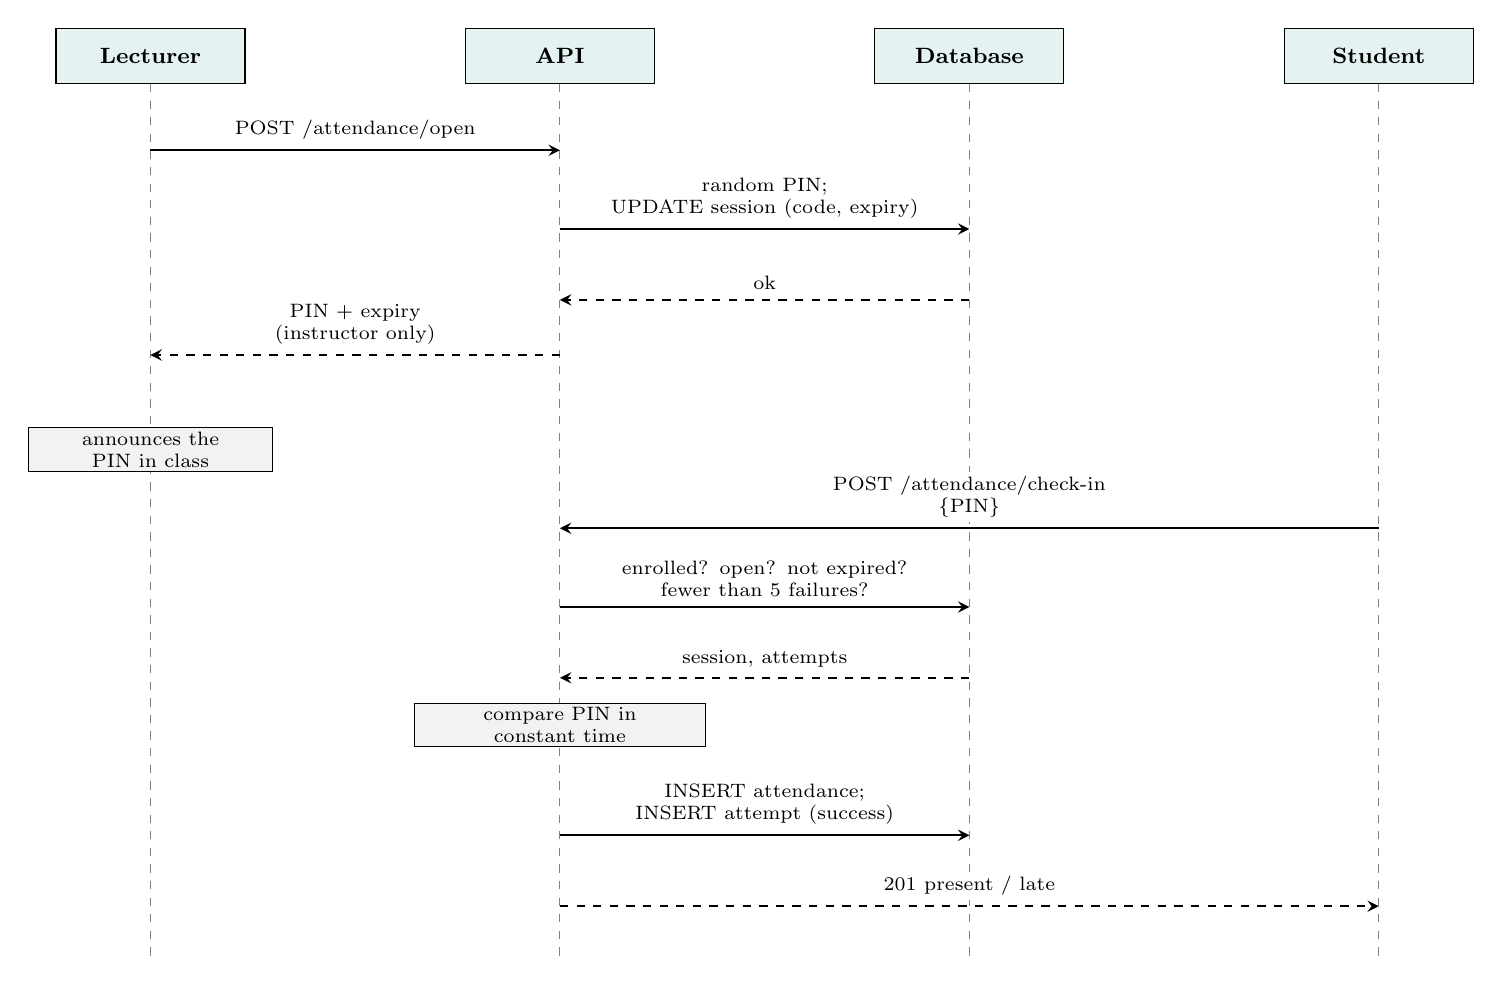
\begin{tikzpicture}[x=1.0cm,y=1.0cm,
    life/.style={dashed, gray},
    head/.style={rectangle, draw, fill=teal!10, minimum width=2.4cm, minimum height=0.7cm, font=\footnotesize\bfseries},
    msg/.style={->, >=stealth, thick},
    lab/.style={font=\scriptsize, fill=white, inner sep=1.5pt, align=center, text width=4.3cm},
    >=stealth]
\node[head] (L) at (0,0) {Lecturer};
\node[head] (A) at (5.2,0) {API};
\node[head] (D) at (10.4,0) {Database};
\node[head] (S) at (15.6,0) {Student};
\foreach \n in {L,A,D,S} \draw[life] (\n) -- ++(0,-11.5);
\draw[msg] (0,-1.2) -- node[lab, above=2pt]{POST /attendance/open} (5.2,-1.2);
\draw[msg] (5.2,-2.2) -- node[lab, above=2pt]{random PIN;\\UPDATE session (code, expiry)} (10.4,-2.2);
\draw[msg, dashed] (10.4,-3.1) -- node[lab, above=2pt]{ok} (5.2,-3.1);
\draw[msg, dashed] (5.2,-3.8) -- node[lab, above=2pt]{PIN + expiry\\(instructor only)} (0,-3.8);
\node[lab, draw, fill=gray!10, text width=3cm] at (0,-5.0) {announces the PIN in class};
\draw[msg] (15.6,-6.0) -- node[lab, above=2pt]{POST /attendance/check-in\\\{PIN\}} (5.2,-6.0);
\draw[msg] (5.2,-7.0) -- node[lab, above=2pt]{enrolled? open? not expired?\\fewer than 5 failures?} (10.4,-7.0);
\draw[msg, dashed] (10.4,-7.9) -- node[lab, above=2pt]{session, attempts} (5.2,-7.9);
\node[lab, draw, fill=gray!10, text width=3.6cm] at (5.2,-8.5) {compare PIN in constant time};
\draw[msg] (5.2,-9.9) -- node[lab, above=2pt]{INSERT attendance;\\INSERT attempt (success)} (10.4,-9.9);
\draw[msg, dashed] (5.2,-10.8) -- node[lab, above=2pt]{201 present / late} (15.6,-10.8);
\end{tikzpicture}}
\caption{Sequence diagram of the PIN attendance (UC6)}
\label{fig:seq-att}
\end{figure}

\subsubsection{State of an Attendance Window}

The window of a session is a small state machine (Figure~\ref{fig:state}). The \texttt{CHECK} constraint of the table makes the invalid combinations unrepresentable: the flag \code{is_attendance_open} is true exactly when both the code and the expiry are present.

\begin{figure}[H]
\centering
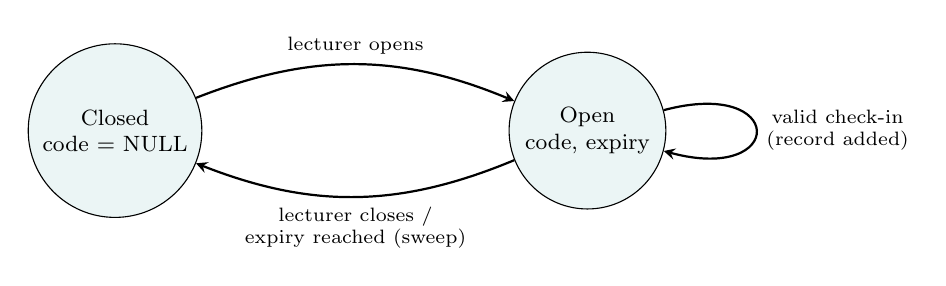
\begin{tikzpicture}[st/.style={circle, draw, fill=teal!8, minimum size=1.7cm, align=center, font=\footnotesize}, >=stealth]
\node[st] (c) at (0,0) {Closed\\code = NULL};
\node[st] (o) at (6,0) {Open\\code, expiry};
\draw[->, thick] (c) to[bend left=22] node[above, font=\scriptsize]{lecturer opens} (o);
\draw[->, thick] (o) to[bend left=22] node[below, font=\scriptsize, align=center]{lecturer closes /\\expiry reached (sweep)} (c);
\draw[->, thick] (o) to[loop right] node[right, font=\scriptsize, align=center]{valid check-in\\(record added)} (o);
\end{tikzpicture}
\caption{State of an attendance window}
\label{fig:state}
\end{figure}

\subsection{Database Design}
\label{sec:db}

\subsubsection{Entity-Relationship Diagram}

Figure~\ref{fig:erd} shows the ERD of the schema. It has fourteen tables: \code{semesters}, \code{courses}, \code{course_classes}, \code{enrollments}, \code{course_sessions}, \code{session_materials}, \code{attendance_records}, \code{attendance_pin_attempts}, \code{users}, \code{skills}, \code{quizzes}, \code{questions}, \code{quiz_interactions} and \code{schema_version}.

\begin{figure}[H]
\centering
\makebox[\textwidth][c]{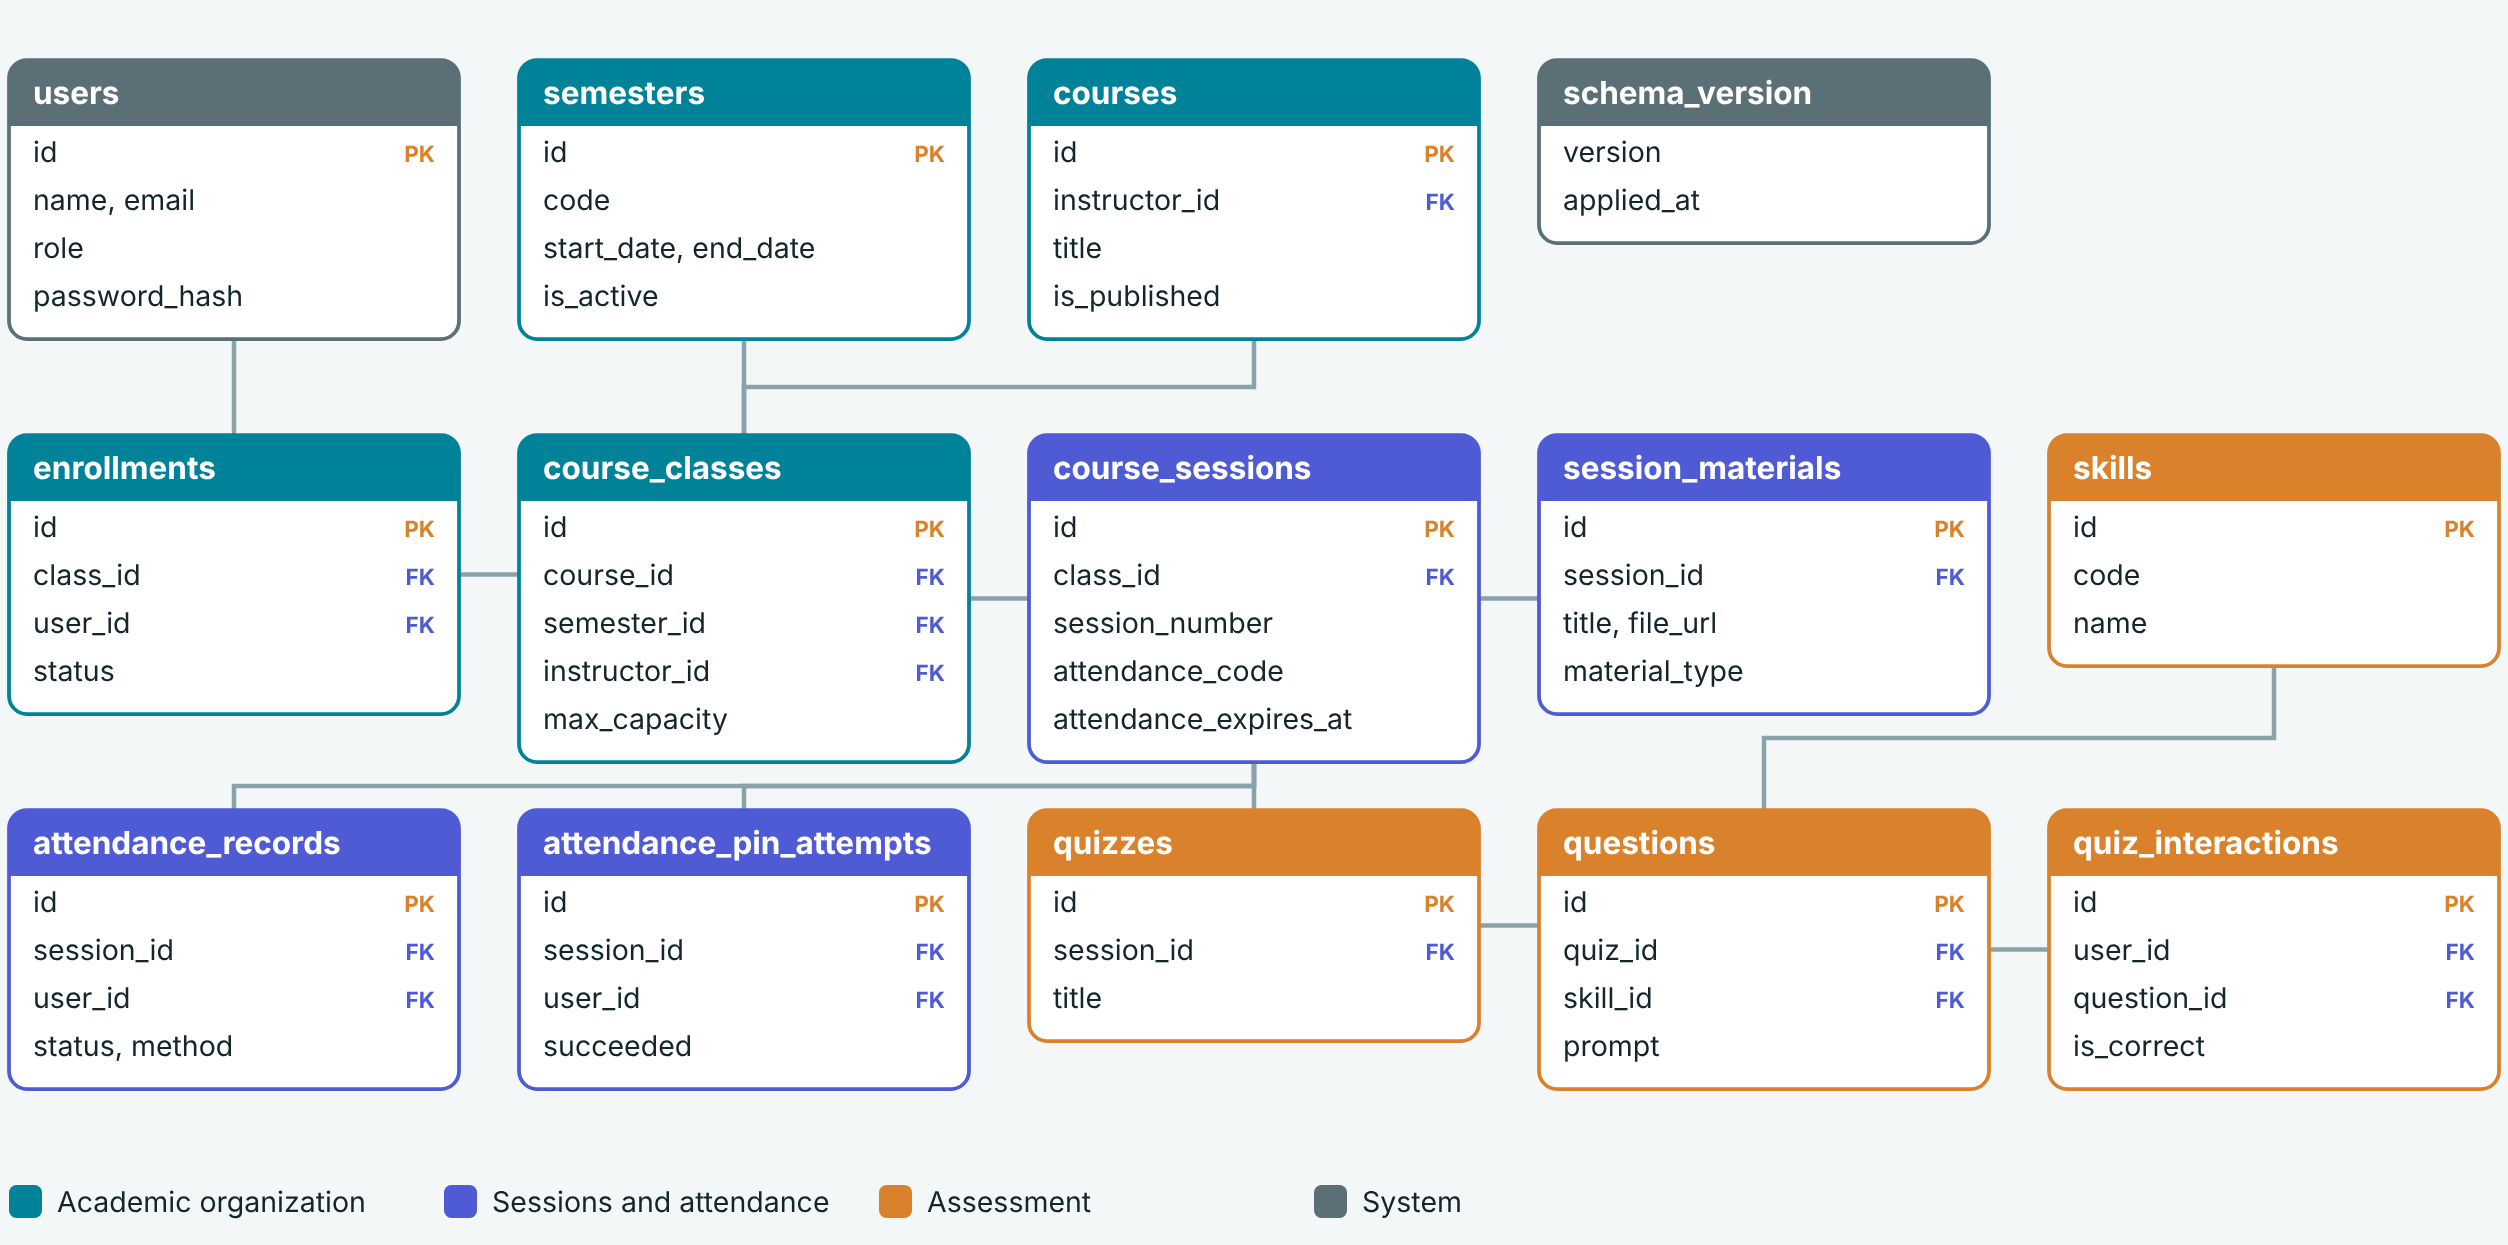
\includegraphics[width=1.18\textwidth]{images/erd.png}}
\caption{Entity-relationship diagram of the database}
\label{fig:erd}
\end{figure}

The central entity is \code{course_classes}: it is an \emph{offering} of a \code{course} in a \code{semester} taught by an instructor. Students are linked to it through \code{enrollments}. A class owns fifteen \code{course_sessions}; each session owns its \code{session_materials}, \code{attendance_records}, \code{quizzes} and \code{attendance_pin_attempts}.

\subsubsection{Data Dictionary}

Tables~\ref{tab:dict1} and~\ref{tab:dict2} summarize the tables. Primary keys are UUIDs generated by \code{gen_random_uuid()}.

\begin{table}[H]
\centering
\caption{Data dictionary (1/2): users, academic structure, schedule}
\label{tab:dict1}
\begin{tblr}{colspec={Q[l,3.3cm]X[l]}, row{1}={font=\bfseries}, hline{1,Z}={0.8pt}, hline{2}={0.4pt}, rowsep=2pt, rows={font=\small}}
Table & Main columns, constraints and meaning\\
\code{users} & \code{name}, \code{email} (unique), \code{password_hash}, \code{role} $\in$ \{student, instructor, admin\}. Self-registration creates students only.\\
\code{semesters} & \code{code} (unique, e.g.\ HK261), \code{name}, \code{start_date}, \code{end_date} with \code{CHECK (start_date <= end_date)}, \code{is_active}; a partial unique index allows at most one active semester.\\
\code{courses} & Catalog entry: \code{instructor_id} (owner), \code{title}, \code{description}, \code{is_published}.\\
\code{course_classes} & An offering: \code{course_id} (cascade), \code{semester_id} (restrict), \code{class_code}, \code{instructor_id} (restrict), \code{max_capacity > 0}, \code{default_room}. \code{UNIQUE (semester_id, class_code)}.\\
\code{enrollments} & \code{class_id}, \code{user_id}, \code{status} $\in$ \{enrolled, dropped\}, \code{enrolled_at}, \code{final_grade} in $[0,100]$. \code{UNIQUE (class_id, user_id)}. Capacity trigger.\\
\code{course_sessions} & \code{class_id}, \code{session_number} in $[1,15]$, \code{title}, \code{session_date}, \code{start_time}, \code{end_time}, \code{room}, and the attendance state: \code{attendance_code}, \code{is_attendance_open}, \code{attendance_expires_at}. \code{UNIQUE (class_id, session_number)}.\\
\code{session_materials} & \code{session_id}, \code{title}, \code{material_type} $\in$ \{slide, code, video\}, \code{file_url}, \code{position}. \code{UNIQUE (session_id, position)}.\\
\end{tblr}
\end{table}

\begin{table}[H]
\centering
\caption{Data dictionary (2/2): attendance, assessment, metadata}
\label{tab:dict2}
\begin{tblr}{colspec={Q[l,3.3cm]X[l]}, row{1}={font=\bfseries}, hline{1,Z}={0.8pt}, hline{2}={0.4pt}, rowsep=2pt, rows={font=\small}}
Table & Main columns, constraints and meaning\\
\code{attendance_records} & \code{session_id}, \code{user_id}, \code{status} $\in$ \{present, absent, late, excused\}, \code{checkin_time}, \code{method} $\in$ \{pin, qr, manual\}, \code{note}. \code{UNIQUE (session_id, user_id)}. Present or late rows must have a time and a method.\\
\code{attendance_pin_attempts} & \code{session_id}, \code{user_id}, \code{attempted_at}, \code{succeeded}. Partial index on failed attempts supports the rate-limit query.\\
\code{skills} & Knowledge component: \code{code} (unique, e.g.\ \code{DSA-LINKEDLIST}), \code{name}, \code{description}.\\
\code{quizzes} & \code{session_id} (required), \code{title}, \code{is_published}.\\
\code{questions} & \code{quiz_id}, \code{skill_id}, \code{prompt}, \code{options} (JSONB), \code{correct_answer} (private), \code{position}. \code{UNIQUE (id, skill_id)} supports the composite foreign key.\\
\code{quiz_interactions} & One row per answer: \code{user_id}, \code{session_id}, \code{question_id}, \code{skill_id}, \code{is_correct}, \code{attempt_count}, \code{created_at}. Composite foreign key \code{(question_id, skill_id)}.\\
\code{schema_version} & Installed schema version, inserted idempotently.\\
\end{tblr}
\end{table}

\subsubsection{Normalization}
\label{sec:normalization}

All tables are in 3NF: each non-key attribute depends on the key only. Examples of design decisions are:

\begin{itemize}
    \item The capacity and the default room belong to the \emph{class}, not to the course, because the same course can be offered with different capacities in different semesters. They are therefore columns of \code{course_classes}.
    \item The enrollment is a separate relation because a student has many classes and a class has many students (many-to-many); \code{status} and \code{final_grade} depend on the pair (class, student).
    \item The skill is stored once in \code{skills}, and \code{questions} refers to it. The redundant \code{skill_id} in \code{quiz_interactions} is a \emph{deliberate} denormalization: it keeps the history of what skill a response was about, and the composite foreign key guarantees that it never differs from the skill of the question.
    \item The attendance state of the current window (\code{attendance_code}, \code{is_attendance_open}, \code{attendance_expires_at}) is stored in \code{course_sessions} because it is a transient attribute of exactly one session and there is at most one active window per session.
\end{itemize}

\subsubsection{Integrity Mechanisms}

\paragraph{Capacity trigger.} Listing~\ref{lst:trigger} shows the trigger function. The statement \texttt{SELECT ... FOR UPDATE} locks the class row, so two concurrent enrollments into the same class are processed one after the other; the second one sees the first. This prevents the anomaly described in Section~\ref{sec:method}~\cite{berenson1995critique, bernstein1981concurrency, postgresdocs}.

\begin{lstlisting}[language=SQLpg, caption={Capacity enforcement trigger (excerpt of \texttt{schema.sql})}, label={lst:trigger}]
CREATE OR REPLACE FUNCTION enforce_course_class_capacity() RETURNS trigger AS $$
DECLARE
  capacity_limit INTEGER;
  current_enrollment_count INTEGER;
BEGIN
  IF NEW.status <> 'enrolled' THEN
    RETURN NEW;
  END IF;
  -- Serialize joins to the same class
  SELECT max_capacity INTO capacity_limit
  FROM course_classes WHERE id = NEW.class_id FOR UPDATE;

  SELECT count(*) INTO current_enrollment_count
  FROM enrollments
  WHERE class_id = NEW.class_id AND status = 'enrolled'
    AND (TG_OP = 'INSERT' OR id <> NEW.id);

  IF current_enrollment_count >= capacity_limit THEN
    RAISE EXCEPTION 'Class capacity has been reached' USING ERRCODE = '23514';
  END IF;
  RETURN NEW;
END;
$$ LANGUAGE plpgsql;
\end{lstlisting}

\paragraph{Window consistency.} Listing~\ref{lst:check} shows the constraints that make an inconsistent attendance state impossible.

\begin{lstlisting}[language=SQLpg, caption={Constraints of \texttt{course\_sessions}}, label={lst:check}]
CHECK (end_time > start_time),
CHECK (attendance_code IS NULL OR attendance_code ~ '^[0-9]{4}$'),
CHECK (is_attendance_open =
       (attendance_code IS NOT NULL AND attendance_expires_at IS NOT NULL))
\end{lstlisting}

\paragraph{Delete behavior.} Deleting a class cascades to its sessions, and from there to materials, attendance, quizzes, interactions and attempts. Deleting a semester or an instructor who still has classes is \emph{restricted}, which protects active offerings from accidental removal. Deleting a skill that is used by a question is restricted.

\subsubsection{Indexes}

The indexes support the queries of the use cases: sessions of a class ordered by date (UC5); enrollments counted by class and status (capacity, UC7); attendance lookup by (user, session); failed PIN attempts of a student in a window (UC6); and interactions by user, skill and time (quiz history).

\subsection{API Design}
\label{sec:api}

Table~\ref{tab:api} lists the endpoints. All endpoints other than registration and login require a valid JWT. Errors use standard HTTP status codes~\cite{rfc9110}; too many failed PIN attempts return 429~\cite{rfc6585}.

\begin{table}[H]
\centering
\caption{REST endpoints of the back end}
\label{tab:api}
\begin{tblr}{colspec={Q[l,1.3cm]Q[l,6.1cm]X[l]}, row{1}={font=\bfseries}, hline{1,Z}={0.8pt}, hline{2}={0.4pt}, rowsep=2pt, rows={font=\small}}
Method & Path & Purpose and access\\
POST & \code{/api/auth/register} & Create a student account\\
POST & \code{/api/auth/login} & Return a one-day JWT\\
GET & \code{/api/schedule?semesterId=} & Sessions of the current user (enrolled or taught), ordered by date and time\\
GET & \code{/api/classes/:classId/sessions} & Sessions and materials of a class; the PIN is visible only to its instructor or an administrator while active\\
POST & \code{/api/classes/:classId/enroll} & Student enrollment; the trigger serializes concurrent joins\\
POST & \code{/api/classes/:classId/sessions} & Instructor creates one session\\
POST & \code{/api/classes/:classId/sessions/bulk} & Instructor creates sessions 1--15 in one transaction\\
POST & \code{/api/sessions/:id/attendance/open} & Open the window for 10--15 minutes (default 10); returns PIN and expiry\\
POST & \code{/api/sessions/:id/attendance/close} & Close the window and clear the PIN\\
POST & \code{/api/sessions/:id/attendance/check-in} & Enrolled student submits \texttt{\{attendanceCode\}}\\
GET & \code{/api/classes/:classId/attendance/summary} & Capacity, enrolled, completed sessions, overall rate, rate per student\\
GET & \code{/api/sessions/:id/quizzes} & Published questions of a session, without the answer key\\
POST & \code{/api/quizzes/:quizId/submit} & Record correctness, skill, attempt and session per question\\
\end{tblr}
\end{table}

\subsection{Security Design}
\label{sec:pin-security}

\subsubsection{Threat Model}

The assets are the integrity of attendance data, the confidentiality of the answer key and the credentials of users. We consider the following threats, which follow the common web risks of~\cite{owasptop10} and the verification requirements of~\cite{owaspasvs}:

\begin{itemize}
    \item a student tries to check in without being in the room (proxy attendance);
    \item a student guesses the PIN by repeated requests;
    \item a user calls an endpoint of a role he or she does not have;
    \item a student reads the answer key from a quiz response;
    \item SQL injection through a request parameter;
    \item two requests race to take the last seat of a class.
\end{itemize}

\subsubsection{Countermeasures}

\begin{table}[H]
\centering
\caption{Threats and countermeasures}
\label{tab:threats}
\begin{tblr}{colspec={Q[l,3.6cm]X[l]}, row{1}={font=\bfseries}, hline{1,Z}={0.8pt}, hline{2}={0.4pt}, rowsep=1.5pt, rows={font=\small}}
Threat & Countermeasure\\
Proxy attendance & The PIN is shown only on the lecturer's screen and expires in 10--15 minutes; a sweep every 15 seconds and a check at check-in both enforce the expiry.\\
PIN guessing & Five failed attempts per student and session in 15 minutes lead to HTTP 429; only enrolled students can try; every attempt is logged in \code{attendance_pin_attempts}; a transaction-level advisory lock on (session, student) serializes parallel requests of the same student so that concurrent guesses cannot bypass the counter.\\
Timing side channel & The submitted PIN is compared with \code{timingSafeEqual} from the Node.js \code{crypto} module, which takes the same time whatever the content.\\
Weak PIN generation & PINs come from \code{randomInt} of \code{node:crypto}, a cryptographically secure generator, not from \code{Math.random}.\\
Privilege escalation & The JWT carries the role; each route checks it; opening and closing attendance and reading the PIN require the instructor of that class or an administrator.\\
Answer-key leakage & The quiz endpoint selects columns explicitly and never returns \code{correct_answer}.\\
Credential theft & bcrypt hashes~\cite{provos1999bcrypt}; JWT with a long private secret read from the environment; tokens expire after one day.\\
SQL injection & Parameterized queries only.\\
Enrollment race & Row lock in the trigger (Listing~\ref{lst:trigger}).\\
\end{tblr}
\end{table}

\subsubsection{Residual Risk of the PIN}

With 10\,000 possible PINs and a limit of five failed attempts in a window, a single student who guesses distinct values has a probability of at most $5/10\,000 = 0.05\%$ of finding the PIN before being blocked. If $k$ students cooperate and each makes five distinct guesses, the probability grows to at most $5k/10\,000$; for $k=10$ it is 0.5\%. The mechanism does not protect against a student who \emph{receives the PIN from a classmate who is present}; no PIN scheme can, and this is why the validity is kept short. For a stronger guarantee the system could add a second factor in the future, for example a one-time code that rotates every minute (Section~\ref{ch:plan}).
